\begin{figure}[H]
    \centering
    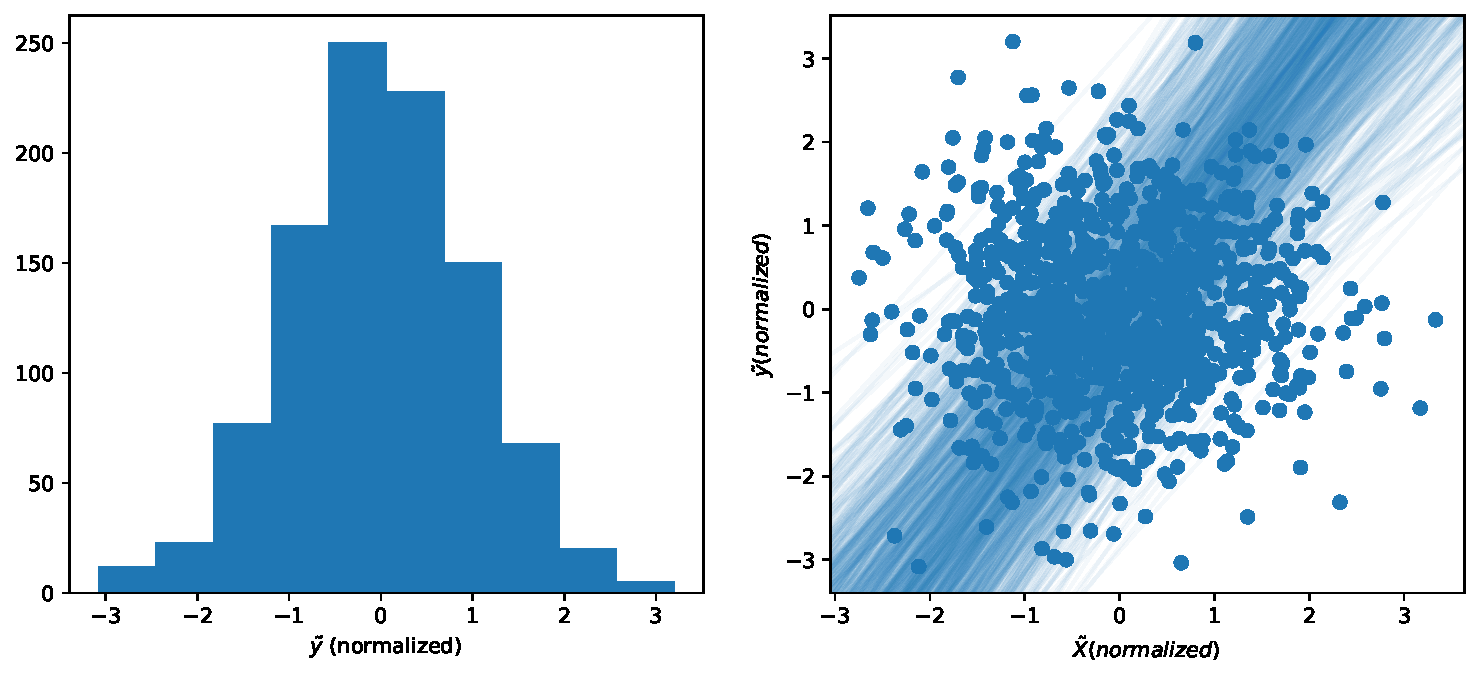
\includegraphics[width=0.8\linewidth]{data/05_reporting/problem_set_2/prior_predictive.pdf}
    \caption{Prior predictive distributions for $\tilde{y}$ and $\mu = \alpha + \beta X_i$ using bootstrapped $\tilde{X} \sim X_i$.}
    \label{fig:prior-predictive}
\end{figure}

Data are normalized before model fitting. Since this is linear regression, we would expect the largest mass of lines ($\mu = \alpha + \beta * X$) to have clear paths through the center of the data, as is seen in Figure \ref{fig:prior-predictive}.